\subsection{UnSupervised Learning - Anamoly Detections}
\label{sec:warmup8}

    There are scenarios in real-life where we have to find anamolies in images. An anamoly can also be find in chest xrays, and using those xrays might generate unsatisfactory results. In this task, we have to find anamolies in chest xrays (if present).

    The basic methodology to tackle this problem is to first get a model to learn features from chest xrays, this can be done using unsupervised learning also if we don't have any labels of the xray. A model having encoder-decoder architecture can be trained to reconstruct the xray. Once trained, the encoder output can be utilized to find anamolies. An image having anamoly will have very different embeddings than a normal image.

\subsubsection{Dataset}
\label{sec:unsupervised-dataset}
  For this task, we were provided dataset having $200$ normal xrays and $17$ abnormal (flipped) xrays. For training, i.e. learning embeddings from a xray, all normal xrays are used, and for testing normal and abnormal xrays are used.

\subsubsection{Training}
 
    An encoder-decoder model with resnet50 as encoder is employed to train to reconstruct the xray. The model is trained with Adam optimizer having learning rate of $10^{-3}$. In initial experiments, MSE loss was utilized as reconstruction loss, but it dodn't gave satisfactory results as the generated xrays failed to generate the ribs and were quite blurry. To overcome this issue, SIMM loss was utilized which uses multiple quantities like luminance, to score the similarity between two images. The model was trained for 20 epochs, and \Cref{fig:reconstruction-learning-curve} shows the validation and training losses for each epochs. 

    \begin{figure}[htbp]
        \centering
        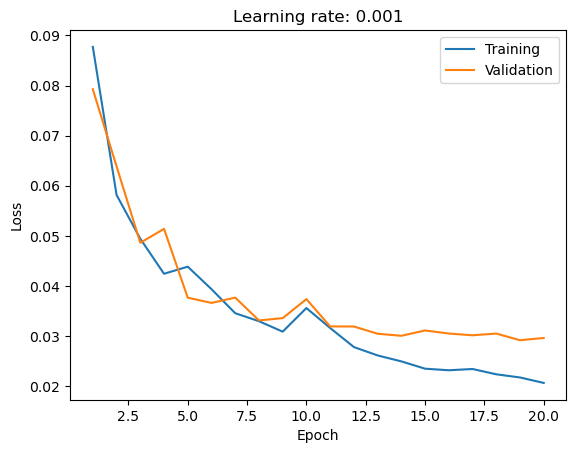
\includegraphics[width=\linewidth]{../plots/unsupervised-anamoly/learning.png}
        \caption{Learning curve of encoder-decoder model with resnet50 as encoder for reconstructing xray images}
        \label{fig:reconstruction-learning-curve}
    \end{figure}


    \subsubsection{Result}
    
    The trained model was able to generate xrays with an average SIMM score of $0.9707$, and \cref{fig:reconstruction-result} shows two reconstructed xrays. The trained model is not able to generate the abnormal images very accurately as it is not able to capture flipped heart and ribs.

    There are two methods in which we can use this model to find anamolies. First, we can use embeddings of encoder to cluster all the embeddings using a clustering algorithm, and find clusters having maximum number of abnormal images. Second, this model can be utilized by anomalib library (\href{https://github.com/openvinotoolkit/anomalib}{github.com/openvinotoolkit/anomalib}) to find anamolies. The first method didn't worked for this model, which might be due to small model.
 
    This model will also be used in \cref{sec:warmup9} for finding orientaion of xrays.
    
    \begin{figure}[htbp]
        \centering
        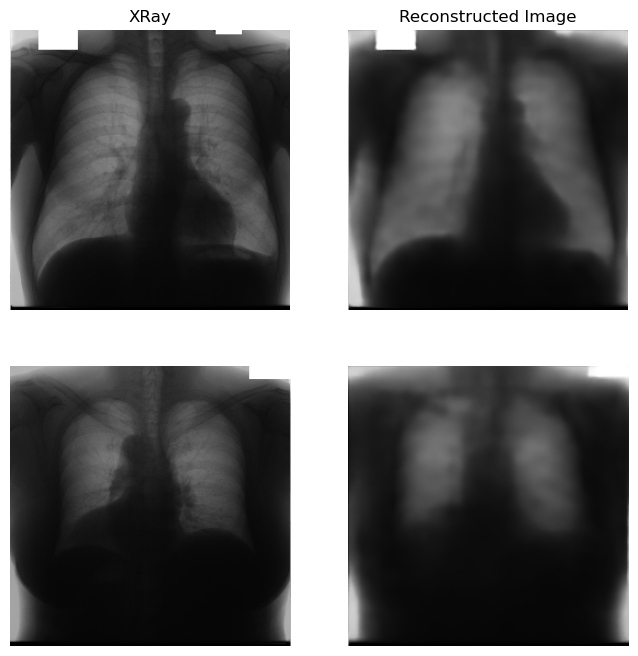
\includegraphics[width=\linewidth]{../plots/unsupervised-anamoly/result.png}
        \caption{Reconstructed xrays of normal and abnormal xrays}
        \label{fig:reconstruction-result}
    \end{figure}